\chapter{Resultados obtenidos}
\label{resul}

\section{Construcción del algoritmo}
El algoritmo diseñado e implementado recibe como parámetros de entrada la cantidad de etapas y la cantidad de nodos de cada una de ellas; además, genera aleatoriamente una matriz de adyacencia con estos datos, luego de calcular el número de nodos, para los cuales también genera aleatoriamente los valores de los \textit{bandits} asociados. Así, la cantidad de etapas y de nodos de cada etapa, serán los valores que el simulador tendrá en cuenta para generar el grafo, verificando que el grupo de aristas sea suficiente para que cada nodo se conecte con al menos uno de la etapa siguiente, así como cumpliendo las demás restricciones de grafo propuesto. 

Cada uno de los nodos del grafo, eventualmente, representa una actividad a desarrollar dentro de una ruta de actividades que debe contener exactamente un nodo de cada etapa del grafo. A cada uno de esos nodos se le ha asociado un \textit{bandit}, que no es otra cosa que un número que indica la recompensa que se obtiene al jugar este \textit{bandit} en un casino, cantidad que para el caso de la simulación será positiva o negativa, pero con magnitud menor a 1; y alrededor de la cual se generan los valores distorsionada que el jugador realmente recibe al seleccionar ese \textit{bandit} en el casino (que casi nunca será el valor real).

Cada \textit{bandit} se genera con una distribución normal con media en cero y desviación estándar de uno; los valores que se generen se consideran los valores reales que debe descubrir el algoritmo. Este valor real será la base para la generación de los valores distorsionados en cada una de las etapas, los cuales se generan tomando ese valor inicial o real como media de otra distribución normal, también con desviación estándar de 1.

En cada algoritmo se calcula una ganancia real, para cada iteración, con los valores reales que se generaron y que corresponden a cada uno de los nodos por donde pase la ruta seleccionada por el algoritmo. También se calcula, para cada iteración la ganancia con los valores distorsionados de la misma ruta, para efectos de poder compararlas eventualmente. Con esta última ganancia es que se harán los cálculos de probabilidades de selección de nodos en las últimas propuestas.

%, con los cuales se calcula la ganancia al final de la ruta, con la que se simula el éxito o el fracaso, de acuerdo al signo de la misma. 

En seguida se presentan las versiones de pseudocódigo que se fueron implementando y probando, las cuales se comparan en su desempeño para dar la mejor como propuesta final.

\subsection{Con probabilidad uniforme}
Inicialmente los nodos de una etapa que sean adyacentes al nodo que ha sido seleccionado en la etapa anterior, tienen una probabilidad uniforme de que seleccionados. 

El pseudocódigo queda como se ve en el cuadro del algoritmo \ref{PsUniforme}, que con los datos de entrada y los generados aleatoriamente para el grafo, calcula una ruta de nodos de cada etapa, solamente teniendo en cuenta que el siguiente forme parte de los vecinos del presente.

\begin{algorithm} [h]
\caption{L-n-bandit-Uniforme(L=Cantidad de etapas, M[L]=Nodos por etapa, n=Cantidad de nodos)} \label{PsUniforme}
\begin{algorithmic}[1]
\STATE Generate: Ad[nxn] = Matriz de adyacencia
\STATE Generate: B[n] = Bandits reales
\FOR{t = 1 \TO T}
     \STATE Initialize: orig = 0
     \STATE Add: orig in path
     \FOR{l = 1 \TO L-1}
        \STATE Generate: $nvz_{orig}$ = vecinos de orig
        \STATE Random: ${dest \in nvz_{orig}}$
        \STATE $orig = dest$
        \STATE Add: orig in path
     \ENDFOR
     \STATE Calculate: $Gan_{path}$
\ENDFOR
\end{algorithmic}
\end{algorithm}

%\begin{figure}
%	\centering
%	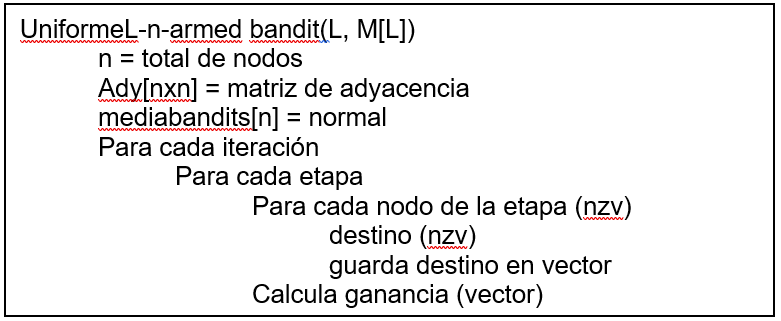
\includegraphics[scale=0.5]{Psuniforme}
%	\caption{Pseudocódigo L-n-armed bandit con Probabilidades Uniformes}
%	\label{PsUniforme}
%\end{figure}

\subsection{Con probabilidades aprendidas}
Posteriormente se implementó el cálculo de la matriz de probabilidades de transición con las fórmulas explicadas en la sección \ref{mat} cuyo pseudocódigo se muestra en el cuadro algorítmico \ref{Pseudo}. A diferencia del anterior, la selección del nodo siguiente al presente en cada ruta, no solo va a tener en cuenta la vecindad con este último, sino el valor que el nodo a seleccionar tenga asociado en la matriz de probabilidad de transición que aquí se genera y se actualiza, de acuerdo a las ganancias que reciba el camino, en cada iteración, como se explica en seguida.

\begin{algorithm}
\caption{L-n-bandit(L=Cantidad de etapas, M[L]=Nodos por etapa, n=Cantidad de nodos)} 
\label{Pseudo}
\begin{algorithmic}[1]
\STATE Initialize: w[n] = 0
\STATE Generate: Ad[nxn] = Matriz de adyacencia
\STATE Generate: B[n] = Bandits reales
\FOR{t = 1 \TO T}
     \STATE Initialize: orig = 0
     \STATE Add: orig in path
     \STATE $P(i \to j) = \frac{e^{v_j}}{\sum_k A_{i,k} e^{v_k}},$
     \FOR{l = 1 \TO L-1}
        \STATE Generate: $nvz_{orig}$ = vecinos de orig
        \STATE Select: ${dest \in nvz_{orig} by P(i \to j)}$
        \STATE $orig = dest$
        \STATE Add: orig in path
     \ENDFOR
     \STATE Calculate: $Gan_{path}$
     \IF{$Gan_{path} > 0$}
        \STATE w[n] = w[n] + $\delta$ by i $\in$ path
     \ENDIF    
\ENDFOR
\end{algorithmic}
\end{algorithm}

Para la primera iteración se maneja una probabilidad uniforme. Para las demás iteraciones, calcula las probabilidades de transición entre nodos y en cada etapa recorre los nodos de una etapa desde la inicial, hasta la penúltima y para cada nodo encuentra sus vecinos o nodos alcanzables, selecciona el que mayor probabilidad de transición presente, o uno al azar cuando aún no estén estipuladas esas probabilidades, para guardarlo en la ruta y proceder a hacer la búsqueda de sus vecinos en la siguiente etapa, con el mismo criterio de selección explicado.

Una vez se conozca la ganancia o pérdida al final de la iteración, se actualizan los valores de preferencia de cada nodo de esa ruta, de acuerdo a la fórmula \ref{model3}, este valor se utiliza para calcular las nuevas probabilidades de transición con la fórmula \ref{model2}, que se tendrán en cuenta en la siguiente iteración. Cabe anotar que al final de cada etapa solo se afectan las probabilidades de transición de los nodos involucrados en la ruta seleccionada, pero que al iniciar cada iteración se cuenta con todas las modificaciones que hayan sufrido estas probabilidades en las iteraciones pasadas de la simulación.

La selección del siguiente vecino está fuertemente influenciada por las probabilidades de transición, constituyéndose en la explotación de los caminos preferidos, pero siempre deja un porcentaje de posibilidad de escoger cualquier nodo que no sea el de mayor probabilidad de transición asociada, lo que permite resolver el problema de la exploración, propio de la teoría de los \textit{bandits}, que garantiza la búsqueda de mejores soluciones que no se han considerado aún.

%Al final de las iteraciones definidas, el simulador converge a la mejor ruta que haya estudiado, que puede ser la óptima. En forma gráfica se puede apreciar esta convergencia en la ganancia que se recibe que al final de las iteraciones tiende a ser una constante. 

%\begin{figure}\label{Pseudo}
%	\centering
%	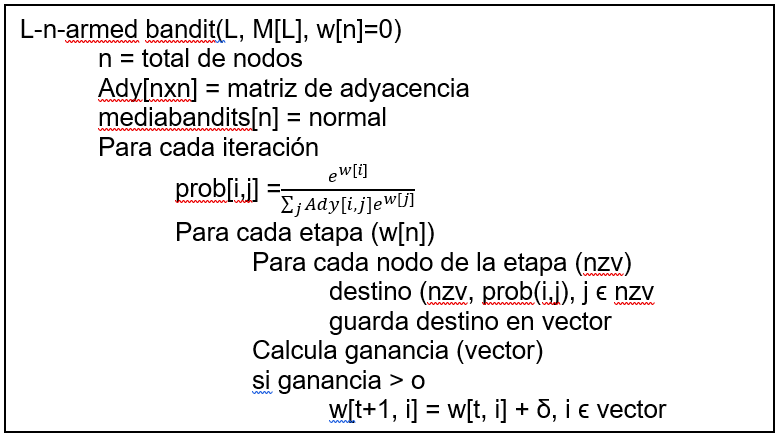
\includegraphics[scale=0.5]{Pseudo}
%	\caption{Pseudocódigo L-n-armed bandit }
%\end{figure}

%El algoritmo recibe los valores de L (número de etapas), M (vector con el número de nodos de cada etapa) y el vector w (valores de preferencia de cada nodo) inicializado en ceros. Calcula n que es la cantidad total de nodos, genera aleatoriamente la matriz de adyacencia y los \textit{bandit} para cada nodo.

%Con los datos de los nodos seleccionados se calcula la ganancia al final de las L etapas de acuerdo a esta se actualizan los valores de preferencia de cada nodo (w) con los que se calcular nuevamente las probabilidades de transición hacia sus vecinos para una nueva iteración.

%\section{PSEUDOCÓDIGO Y PRUEBAS}

%Inicialmente se toma un grafo modelo que se presenta en la figura \ref{Grafomodelo} con su matriz de adyacencia y valores de sus \textit{bandits} fijos. Se le da libertad a los algoritmos a evaluar, que decidan las rutas a seguir de forma aleatoria.

%\begin{figure}[H]
%\label{Grafomodelo}
%	\centering
%	\includegraphics[scale=0.5]{Grafomodelo}
%	\caption{Grafo de 5 etapas con 13 nodos}
%	\label{Pseudocódigo}
%\end{figure}

%El desempeño del algoritmo propuesto se compara con un algoritmo que asigna probabilidades uniformes a las transiciones entre un nodo y sus vecinos, quedando la decisión del nodo a seguir al azar. El pseudocódigo correspondiente se ve en el cuadro \ref{PsUniforme}. Como era de esperarse, la convergencia hacia una buena solución no se refleja como en el algoritmo propuesto.

\subsection{Calculando promedios de ganancias}

También se implementa un algoritmo que evalúa el resultado al estilo de \textit{Q-learning}, pero donde la selección no se hace sobre un conjunto de acciones, sino sobre un conjunto de rutas de acciones de las que ha explorado alguna vez, cuyo pseudocódigo se muestra en el cuadro del algoritmo \ref{PsQ-learning}. 

Aquí se aprovecha el constructo algorítmico ya diseñado, para la selección de los nodos, de acuerdo a unas probabilidades de transición que se van generando de acuerdo a su participación en una ruta con ganancia o con pérdida, por lo que se siguen realizando todos los cálculos matemáticos e instrucciones que este constructo conlleva. La diferencia fundamental está en la forma como se define la respuesta.

\vspace{1cm}
\begin{algorithm} []
\caption{L-n-bandit(L=Cantidad de etapas, M[L]=Nodos por etapa, n=Cantidad de nodos)} 
\label{PsQ-learning}
\begin{algorithmic}[1]
\STATE Initialize: w[n] = 0
\STATE Generate: Ad[nxn] = Matriz de adyacencia
\STATE Generate: B[n] = Bandits reales
\FOR{t = 1 \TO T}
     \STATE Initialize: orig = 0
     \STATE Add: orig in path
     \STATE $P(i \to j) = \frac{e^{v_j}}{\sum_k A_{i,k} e^{v_k}},$
     \FOR{l = 1 \TO L-1}
        \STATE Generate: $nvz_{orig}$ = vecinos de orig
        \STATE Select: ${dest \in nvz_{orig} by P(i \to j)}$
        \STATE $orig = dest$
        \STATE Add: orig in path
     \ENDFOR
     \STATE Calculate: $Gan_{path}$
     \IF{$Gan_{path} > 0$}
        \STATE w[n] = w[n] + $\delta$ by i $\in$ path
     \ENDIF   
     \STATE Calculate: $Ganprom_{path}$
\ENDFOR
\STATE Select: Max Ganprom$\{$x$\}$
\STATE Print: Path = Arg(x) 
\end{algorithmic}
\end{algorithm}

%\begin{figure}\label{PsQ-learning}
%	\centering
%	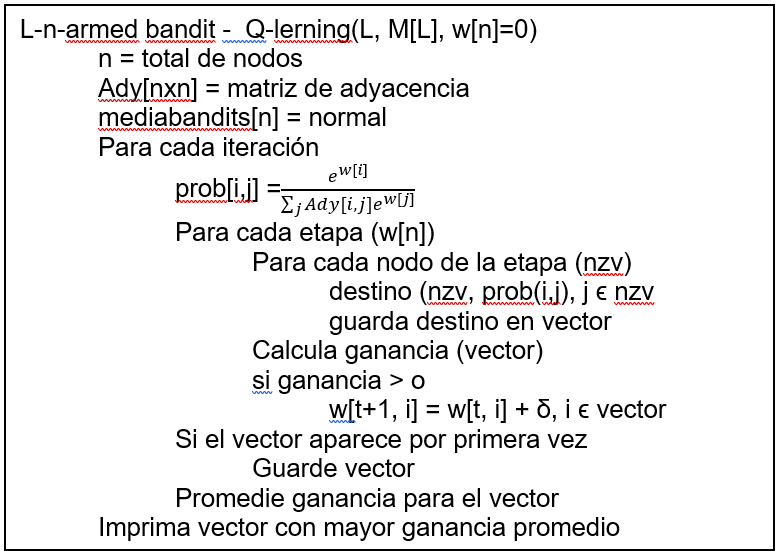
\includegraphics[scale=0.5]{PsQ-learning}
%	\caption{Pseudocódigo L-n-armed bandit – Q-learning}
%	\label{PsQ-learning}
%\end{figure}


En esta propuesta, la aplicación debe ir guardando en un arreglo cada una de las rutas nuevas que se van generando por iteración, junto con su ganancia calculada, porque si la ruta no es nueva, solo debe incrementar un contador que hace parte del mismo arreglo. De esta manera, al finalizar cualquier cantidad de iteraciones, se calculará la ganancia promedio para cada ruta generada, parámetro en el que se basa para seleccionar la ruta con mejor ganancia promedio y presentarla como la óptima.

Las pruebas correspondientes se presentan en el capítulo \ref{resul} donde se detallan los resultado que se fueron obteniendo en algoritmos previos y en los que finalmente se comparan.

\section{Pruebas}

\subsection{Generador de bandits}

Primero se probó el algoritmo que genera los \textit{bandits} para los nodos y aplica la fórmula de los promedios de las ganancias para entregar al final la acción con mejor valor asociado, dándole al algoritmo valores distorsionados que se encontraban entre una desviación estándar de 1 del valor asociado al \textit{bandit}. Este código se probó varias veces y siempre encontró el valor buscado. 

La figura \ref{AlgBandit} es el resultado gráfico de una corrida de este algoritmo con 400 iteraciones, donde la línea roja representa las ganancias que va encontrando en cada iteración y la línea horizontal que está ubicada en 1 representa el número del brazo que en promedio obtiene la mejor ganancia al finalizar las iteraciones, respuesta que corresponde exactamente con el \textit{bandit} que tiene asignado el mayor valor de ganancia real, de los 10 que se le dieron a escoger.

\begin{figure} [H]
    \label{Resul2}
	\centering
	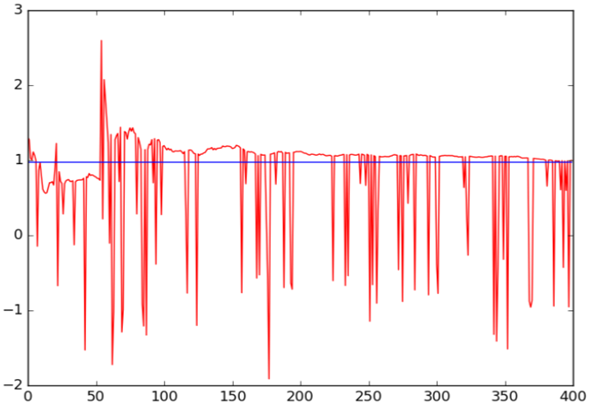
\includegraphics[scale=0.6]{AlgBandit}
	\caption{Resultado de la selección del mejor brazo usando la teoría de los \textit{bandits}}
	\label{AlgBandit}
\end{figure}

La oscilación de la línea roja se produce por la exploración que el algoritmo hace de otras alternativas diferentes a la que en cada momento parece ser la mejor. Tampoco dan los mismos valores aunque esté probando el mismo brazo, porque estos valores están siendo generado con una distribución normal, con media en uno real (que también fue aleatorio), pero dentro de una desviación estándar que en este caso fue de 1. 

\subsection{Generador de la matriz de adyacencia}

Posteriormente se implementó el código que genera las matrices de adyacencia del grafo por etapas. Estas matrices debían ser escalonadas, debían obedecer a los requisitos de precedencia de nodos entre etapas y debía tener al menos un 1 en cada fila para garantizar la conexión de las etapas. Este código también se probó varias veces y siempre arrojó resultados adecuados. Un ejemplo de este resultado se muestra en la figura \ref{MatrizAy}.

\begin{figure} [H]
    \label{Resul2}
	\centering
	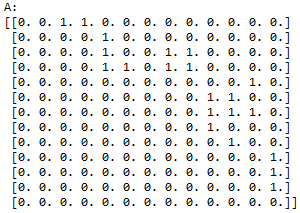
\includegraphics[scale=0.8]{MatrizAy}
	\caption{Resultado de la matriz de adyacencia para un grafo por etapas}
	\label{MatrizAy}
\end{figure}

\subsubsection{Generación de una ruta aleatoria}

Se implementó la fusión del algoritmo para la generación de la matriz de adyacencia, con el que genera los valores asociados a cada nodo o \textit{bandit}; el pseudocódigo correspondiente se probó con valores aleatorios, obteniendo siempre la matriz escalonada que se esperaba y los valores asociados a los \textit{bandits}.

Se le adicionó la funcionalidad de que tomara una ruta factible, teniendo en cuenta la matriz de adyacencia para tomar la información de los posibles vecinos de cada nodo. La pruebas que se hicieron funcionaron siempre correctamente.

Se procedió a probar que sobre la ruta que seleccionara calculara correctamente la ganancia real asociada, teniendo en cuenta el vector de valores generados para los \textit{bandits}, y la ganancia distorsionada asociada a esa misma ruta, teniendo en cuenta el nuevo vector de valores distorsionados de los \textit{bandits}, el cual se genera con números aleatorios que siguen una distribución normal con media en el elemento del primer vector, dentro de una desviación estándar de 1. Las pruebas para esta implementación siempre funcionaron correctamente.

\subsection{Encontrando la ruta óptima}

Aquí se dan tres momentos diferentes: Inicialmente el que ya está implementado, donde la escogencia del siguiente nodo de un camino, solo tiene que estar dentro del conjunto de vecinos del nodo actual, pero todos con la misma probabilidad de ser seleccionados; a este modelo le reconoceremos como Probabilidades Uniformes. Seguidamente se implementa la generación de la matriz de probabilidades de transición de pasar de un nodo a otro, la cual se basa en un fundamento matemático específico que se presentó en la sección \ref{mat} y del que se espera que converja a una única respuesta con la mejor ruta encontrada; a este le reconoceremos como Probabilidad Modelada. Finalmente, y en forma paralela con el desarrollo del algoritmo anterior, se implementa una funcionalidad que permite seleccionar la ruta que, durante todas las iteraciones, alcanzó el mayor promedio de ganancias, para entregarla como respuesta; este algoritmo lo reconoceremos como Promedio de Ganancias.

\subsection{Búsqueda con Probabilidad Uniforme}

Este algoritmo se construye básicamente, incluyendo un contador de iteraciones para que el algoritmo de generación de rutas factibles se ejecute una cantidad dada de veces determinada y una selección de la ruta que al final de las iteraciones hubiera obtenido la ganancia promedio, para entregarla como respuesta. 

Inicialmente los valores de la matriz de adyacencia y del vector de \textit{bandits} se generaron de forma aleatoria con las instrucciones que ya estaban probadas y que se describieron anteriormente, pero esto no permitía estimar la efectividad del algoritmo, porque, en muchos casos, no eran significativamente diferentes los valores asignados a los nodos y cualquier ruta era buena. 

\subsubsection{Grafo para las pruebas}

Se decide entonces trabajar con un grafo de 5 etapas y 13 nodos, dispuestos como se ve en la figura \ref{Grafomodelo}, pero no necesariamente con esas aristas, es decir, con matriz de adyacencia aleatoria, así como los valores de sus \textit{bandits}, pero obligando a que uno de ellos por etapa tuviese un mayor valor que los demás, para favorecer la ruta mejor y así verificar si estaba funcionando.

\begin{figure}[h]
  \centering
    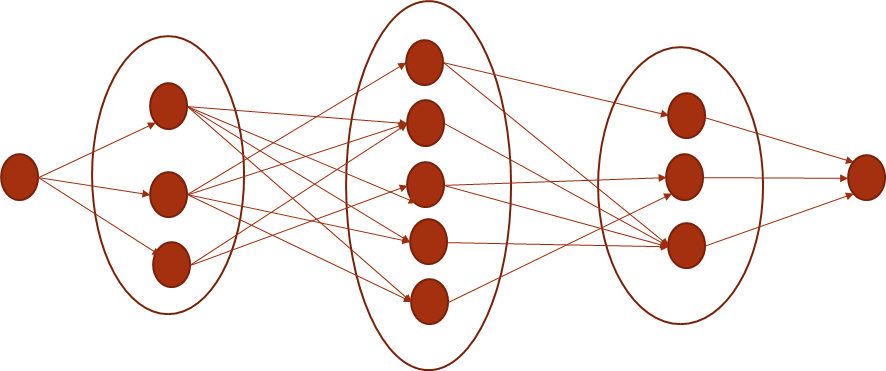
\includegraphics[scale=0.5]{GrafoModelo.png}
  \caption[Grafo Modelo]{Grafo Modelo con 5 etapas y 13 nodos}
  \label{Grafomodelo}
\end{figure}

De otra parte, era importante saber cómo se comportaba el algoritmo, al ejecutarlo varias veces, dejando fijos los datos de entrada correspondientes al grafo que se quería evaluar, por lo que de aquí en adelante no se generaron más matrices de adyacencia ni vectores reales de los \textit{bandits} aleatorios, sino que se dejaron los siguientes:

\renewcommand{\arraystretch}{0.5}
%\begin{equation}
A = 
$\begin{bmatrix}
%\hspace{2cm}

0, 0, 1,  1,  0,  0,  0,  0,  0,  0,  0,  0,  0\\
0, 0, 0,  0,  1,  0,  0,  0,  0,  0,  0,  0,  0\\
0, 0, 0,  0,  1,  0,  0,  1,  1,  0,  0,  0,  0\\
0, 0, 0,  0,  1,  1,  0,  1,  1,  0,  0,  0,  0\\
0, 0, 0,  0,  0,  0,  0,  0,  0,  0,  0,  1,  0\\
0, 0, 0,  0,  0,  0,  0,  0,  0,  1,  1,  0,  0\\
0, 0, 0,  0,  0,  0,  0,  0,  0,  1,  1,  1,  0\\
0, 0, 0,  0,  0,  0,  0,  0,  0,  1,  0,  0,  0\\
0, 0, 0,  0,  0,  0,  0,  0,  0,  0,  1,  0,  0\\
0, 0, 0,  0,  0,  0,  0,  0,  0,  0,  0,  1,  0\\
0, 0, 0,  0,  0,  0,  0,  0,  0,  0,  0,  1,  0\\
0, 0, 0,  0,  0,  0,  0,  0,  0,  0,  0,  1,  0\\
0, 0, 0,  0,  0,  0,  0,  0,  0,  0,  0,  0,  0
\end{bmatrix}$

%\end{equation}

%\begin{figure}
%	\centering
%	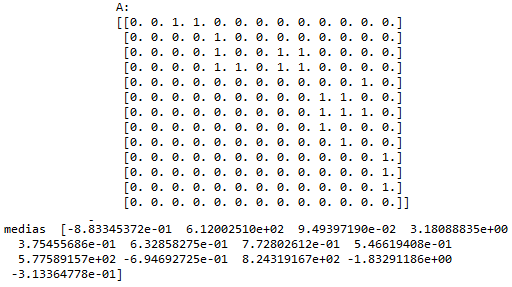
\includegraphics[scale=1]{MatrizAyBandits2}
%	\caption{Matriz y bandit generados}
%	\label{AyB}
%\end{figure}

B = [- 0.833e-01, 6.12e+02, 9.49e-02, 3.18e+00, 3.75e-01, 6.33e-01, 7.73e-01, 5.47e-01, 5.77e+02, -6.95e-01, 8.23e+02, -1.83e+00, -3.13e-01]

\subsubsection{Resultados probabilidad uniforme}

El algoritmo cuyo pseudocódigo se presentó en el cuadro \ref{PsUniforme}, se ejecutó con 99 intervalos de tiempo. La figura \ref{fig:uniforme} muestra uno de los resultados. 

\begin{figure}[H]
	\centering
	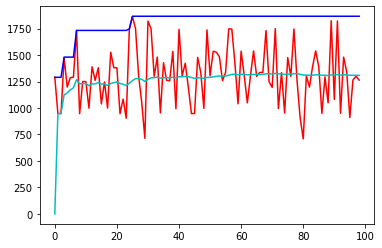
\includegraphics[scale=1]{Uniforme}
	\caption{Resultado con probabilidad uniforme}
	\label{fig:uniforme}
\end{figure}

En esta gráfica, la curva superior azul corresponde a la ganancia de la mejor ruta probada hasta el momento, calculada con el valor real de los \textit{bandits} o medias asignadas a cada uno; en la curva más inestable se presentan las ganancias obtenidas en cada instante de tiempo por la ruta seleccionada, calculada con los valores distorsionados de los \textit{bandits}, que fueron generados alrededor del vector B de las medias, con una desviación estándar de 1; y en la curva inferior verdosa se muestra el promedio acumulado de estas ganancias, el cual converge a un único valor a través del tiempo, pero no trata de acercarse al valor real.

\subsection{Resultados probabilidad modelada}

Para 33 iteraciones, T=33 en el algoritmo que se muestra en el cuadro \ref{Pseudo}, para las cales se pueden apreciar los valores que van tomado sus variables para construir la matriz de probabilidades de transición, la ganancia promedio generada por el algoritmo, convergió rápidamente hacia el valor de la mejor ganancia real como se puede apreciar en la figura \ref{Resul2}. 

\begin{figure} [H]
	\centering
	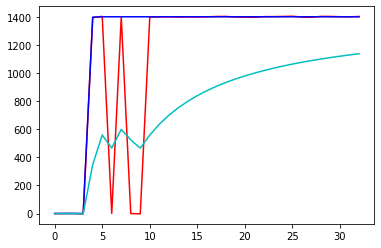
\includegraphics[scale=1]{Resul2}
	\caption{Resultado con probabilidad ponderada semialeatorio}
	\label{Resul2}
\end{figure}

En esta gráfica, al igual que en la del modelo anterior, la curva superior azul corresponde a la ganancia de la mejor ruta probada hasta el momento, calculada con el valor real de los \textit{bandits} o medias asignadas a cada uno; en la curva más inestable se presentan las ganancias obtenidas en cada instante de tiempo por la ruta seleccionada, calculada con los valores distorsionados de los \textit{bandits}, que fueron generados alrededor del vector B de las medias, con una desviación estándar de 1; y en la curva inferior verdosa se muestra el promedio acumulado de estas ganancias.

\subsection{Resultados selección de la ruta con mayor ganancia promedio}

También se implementa un algoritmo que evalúa el resultado al estilo de \textit{Q-learning}, pero donde la selección no se hace sobre un conjunto de acciones, sino sobre un conjunto de rutas de acciones de las que ha explorado alguna vez, cuyo pseudocódigo se muestra en el cuadro algorítmico \ref{PsQ-learning}. Para garantizar una comparación válida, este algoritmo se incorpora en el mismo código del algoritmo anteriormente presentado, lo que asegura que se manejan los mismos datos y que las decisiones que se toman de forma aleatoria serán las mismas. 

El 100\% de las veces que se probó, encontró la ruta óptima. No se generan gráficas para este algoritmo, puesto que no se haya un único promedio de ganancias, sino que se promedia para cada una de las rutas que el algoritmo encuentra, de forma que el criterio de selección de la ruta óptima no tiene que ver con convergencia alguna.

%\section{Pruebas de los algoritmos propuestos} 

%\section{GENERACIÓN DE DATOS ALEATORIOS}
%Al rededor de los valores dados a cada uno de los nodos del grafo, la aplicación genera valores distorsionados con una diferencia de más o menos uno, generados en forma aleatoria, siendo diferentes los valores que se obtienen en cada ejecución.

%Así mismo, todos los nodos tienen la misma probabilidad de ser elegidos cuando se hace la primera corrida, así que la aplicación hace las selecciones en cada etapa, mediante la generación de un valor aleatorio con distribución uniforme; para los demás tiempos de corridas, en que los nodos ya cuentan con valore asociados, el nodo que selecciona dentro de los vecinos de un nodo cualquiera, atendiendo a las probabilidades de transición que se le ofrecen, en forma de ruleta donde el ancho de las franjas para cada opción es equivalente al la probabilidad misma.

%Estos valores distorsionados, con los que realmente decide el jugador y, por ende, trabaja la aplicación, han sido calculados sumándole al número que indica la recompensa real, una cantidad aleatoria generada con una distribución normal con media en 0 y una desviación estándar de 1, es decir que se le suma a la media una cantidad entre -1 y +1.

\section{Comparación entre Probabilidad Modelada y Mayor ganancia promedio} 

Estos dos algoritmos han logrado encontrar la ruta óptima del grafo elegido. Aquí presentamos los resultados de los dos, ejecutándolos en el mismo programa, para que los valores que se generan aleatoriamente sean los mismos y darle de esta forma validez a la comparación.

Se toma el grafo modelo que se presenta en la figura \ref{Grafomodelo} con su matriz de adyacencia fija, así como los valores para sus \textit{bandits}, que ya se escribieron anteriormente, de forma que cualquier resultada se pueda comparar con los de otros algoritmos y con ejecuciones posteriores del mismo algoritmo. Se le da libertad al algoritmo para generar aleatoriamente los valores distorsionados de los \textit{bandit} que simula la incertidumbre del ejercicio, al no conocerse los valores reales. Finalmente, el algoritmo decide los nodos que selecciona en cada etapa y, así, las rutas a seguir también serán aleatorias.

La decisión de usar una generación de números aleatorios que siguen una distribución normal con media en cero y desviación estándar en 1, es porque es la utilizada en la literatura de aprendizaje por refuerzo \citep{sutton1992reinforcement}, con la cual se ha probado el funcionamiento del modelo de decisión n-armed bandit. 

%Para demostrar la importancia que tiene el modelo de la generación de probabilidades de transición de estados entre los nodos, se corrió una aplicación donde los nodos se seleccionan todo el tiempo al azar, respetando las posibilidades de adyacencia del grafo, y se comparan sus resultados con una ejecución del algoritmo que genera y tiene en cuenta las probabilidades mencionadas.

Con un $\delta$ de aprendizaje de 0.0003 multiplicado por el valor de la ganancia o recompensa de la ruta utilizada, Se hicieron 10 corridas al algoritmo de probabilidades de transición, el cual permite que, a lo largo de todas las corridas o ejecuciones del algoritmo, se vaya aumentando la probabilidad de que cada nodo sea escogido.

Para cada ejecución se ha seleccionado la última respuesta que arrojó la aplicación en cada una de las dos modalidades expuestas donde, para el caso del algoritmo de Probabilidad modelada, fue la que se obtuvo cuando el algoritmo convergió, haciendo uso de la fórmula \ref{model2}, como se explicó en la sección \ref{implemodprob}, mientras que para el caso de algoritmo de Mayor ganancia promedio, esta respuesta es la que se va dando al terminar cada iteración. 

Los resultados obtenidos se muestran en la tabla \ref{tabComUP}, en los cuales se puede establecer que el 70\% de las veces que se probó el algoritmo de Probabilidad modelada, encontró la ruta óptima y que el 100\% de las veces que se probó el algoritmo de Mayor ganancia promedio, este encontró la ruta óptima.

\renewcommand{\arraystretch}{0.5}
\begin{table}[H] 
\centering
\caption{Comparación de resultados de los dos enfoques} \begin{tabular}{ccc}
\hline
\begin{tabular}[c]{@{}c@{}}Número de \\ Corrida\end{tabular} & \begin{tabular}[c]{@{}c@{}}Con el modelo \\ de probabilidades\end{tabular} & \begin{tabular}[c]{@{}c@{}}Con el simulador \\ de bandits de vectores\end{tabular} \\[0.5ex] \hline
1                           & {[}0, 2, 4, 11, 12{]}                               & {[}0, 2, 4, 11, 12{]}                                       \\
2                           & {[}0, 2, 5, 11, 12{]}                               & {[}0, 2, 4, 11, 12{]}                                       \\
3                           & {[}0, 2, 4, 11, 12{]}                               & {[}0, 2, 4, 11, 12{]}                                       \\
4                           & {[}0, 2, 4, 11, 12{]}                               & {[}0, 2, 4, 11, 12{]}                                       \\
5                           & {[}0, 2, 4, 11, 12{]}                               & {[}0, 2, 4, 11, 12{]}                                       \\
6                           & {[}0, 2, 4, 11, 12{]}                               & {[}0, 2, 4, 11, 12{]}                                       \\
7                           & {[}0, 2, 4, 11, 12{]}                               & {[}0, 2, 4, 11, 12{]}                                       \\
8                           & {[}0, 2, 7, 11, 12{]}                               & {[}0, 2, 4, 11, 12{]}                                       \\
9                           & {[}0, 2, 4, 11, 12{]}                               & {[}0, 2, 4, 11, 12{]}                                       \\
10                          & {[}0, 2, 7, 11, 12{]}                               & {[}0, 2, 4, 11, 12{]}                                 
\end{tabular}
\label{tabComUP}
\end{table}

Adicionalmente a los resultados que se muestran en la tabla \ref{tabComUP}, se pueden observar las figuras generadas por la aplicación el la figura \ref{fig:grafi}. Allí, la curva superior, que se dejó en color verde, representa la ganancia de la mejor ruta probada hasta ese momento, calculada con los valores reales de los \textit{bandits} ya dados en el vector B. Esto permite que el software sea el que estime la mejor ruta, de un conjunto aleatorio de nodos, sin una intervención manual, ya que hacer este cálculo equivaldría a una búsqueda exhaustiva en árbol, lo que puede llegar a ser muy dispendioso.

Seguidamente, en la curva más variable (roja) se presentan las ganancias obtenidas en cada una de las iteraciones por la ruta allí seleccionada, calculada con los valores distorsionados de los \textit{bandits}, que fueron generados alrededor de las medias reales con desviación estándar de 1. 

Y, por último, en la curva inferior (azul) se muestra el promedio acumulado de estas ganancias, el cual converge a un único valor a través del tiempo y se espera que se acerque al valor real de la mejor ruta, representado en la línea superior.

Se ejecuta el código 10 veces consecutivas para obtener una estimación inicial de su efectividad, cada vez con 999 iteraciones.

Los resultados obtenidos entregan el vector de nodos de las L etapas que ofrece la mayor ganancia, como es [0,2,4,11,12], para los dos modelos, que, en este caso, se puede verificar manualmente.

Como en otras oportunidades, se obtiene solo un porcentaje de siete de diez ejecuciones que llevan a la respuesta correcta siguiendo el procedimiento de generación aproximada de la matriz de transición de probabilidades, como se puede apreciar en la figura compuesta \ref{fig:grafi} y en la tabla \ref{tabComUP}. %el apéndice \ref{resultProb10}%.

\begin{figure} 
    \centering
    \begin{subfigure}[b]{0.39\textwidth}
        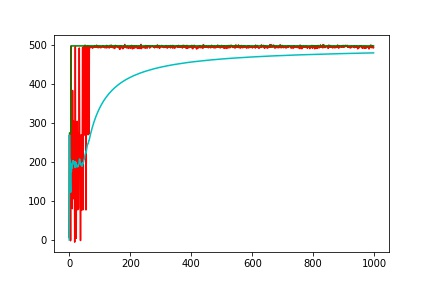
\includegraphics[width=\textwidth]{grafi1.jpg}
        %\caption{A gull}
        \label{fig:gull}
    \end{subfigure}
    \vspace{0.5 mm}
    ~ %add desired spacing between images, e. g. ~, \quad, \qquad, \hfill etc. 
      %(or a blank line to force the subfigure onto a new line)
    \begin{subfigure}[b]{0.39\textwidth}
        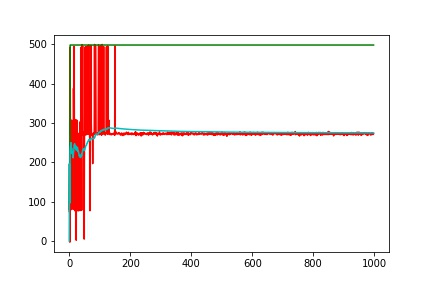
\includegraphics[width=\textwidth]{grafi2.jpg}
        %\caption{A tiger}
        \label{fig:tiger}
    \end{subfigure}
    ~ %add desired spacing between images, e. g. ~, \quad, \qquad, \hfill etc. 
    %(or a blank line to force the subfigure onto a new line)
    \begin{subfigure}[b]{0.39\textwidth}
        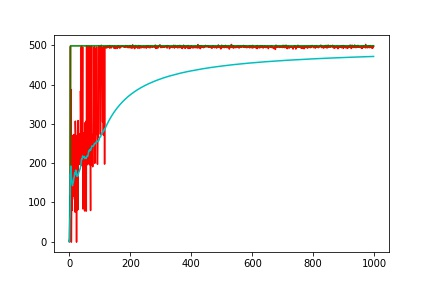
\includegraphics[width=\textwidth]{grafi3.jpg}
        %\caption{A mouse}
        \label{fig:mouse}
    \end{subfigure}
    \begin{subfigure}[b]{0.39\textwidth}
        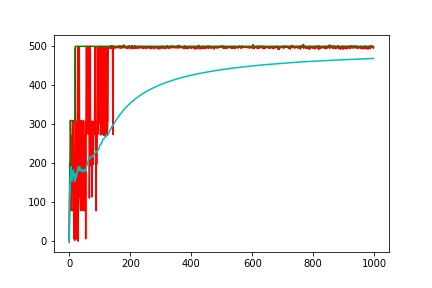
\includegraphics[width=\textwidth]{grafi4.jpg}
        %\caption{A tiger}
        \label{fig:tiger}
    \end{subfigure}
        \begin{subfigure}[b]{0.39\textwidth}
        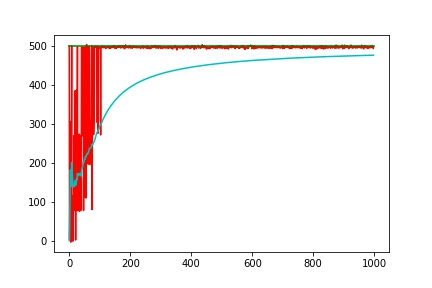
\includegraphics[width=\textwidth]{grafi5.jpg}
        %\caption{A gull}
        \label{fig:gull}
    \end{subfigure}
    ~ %add desired spacing between images, e. g. ~, \quad, \qquad, \hfill etc. 
      %(or a blank line to force the subfigure onto a new line)
    \begin{subfigure}[b]{0.39\textwidth}
        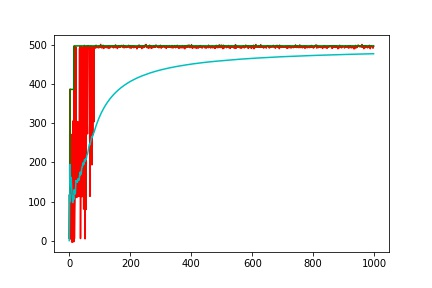
\includegraphics[width=\textwidth]{grafi6.jpg}
        %\caption{A tiger}
        \label{fig:tiger}
    \end{subfigure}
    ~ %add desired spacing between images, e. g. ~, \quad, \qquad, \hfill etc. 
    %(or a blank line to force the subfigure onto a new line)
    \begin{subfigure}[b]{0.39\textwidth}
        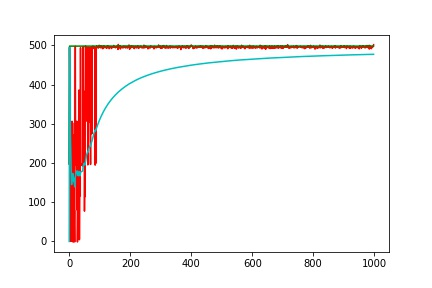
\includegraphics[width=\textwidth]{grafi7.jpg}
        %\caption{A mouse}
        \label{fig:mouse}
    \end{subfigure}
    \begin{subfigure}[b]{0.39\textwidth}
        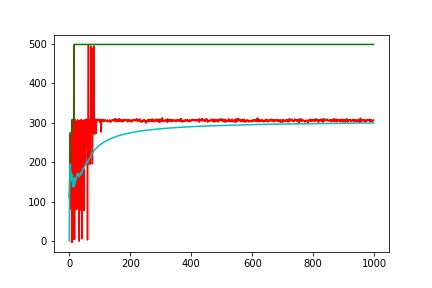
\includegraphics[width=\textwidth]{grafi8.jpg}
        %\caption{A tiger}
        \label{fig:tiger}
    \end{subfigure}
    \begin{subfigure}[b]{0.39\textwidth}
        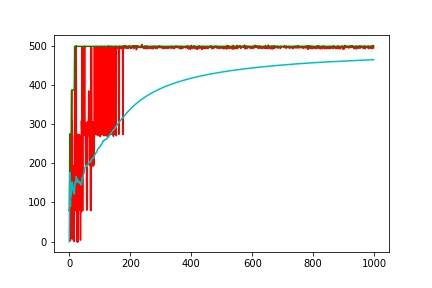
\includegraphics[width=\textwidth]{grafi9.jpg}
        %\caption{A mouse}
        \label{fig:mouse}
    \end{subfigure}
    \begin{subfigure}[b]{0.39\textwidth}
        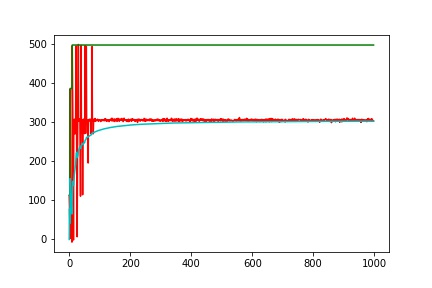
\includegraphics[width=\textwidth]{grafi10.jpg}
        %\caption{A tiger}
        \label{fig:tiger}
    \end{subfigure}    
    \caption{Ejecución algoritmo Probabilidad Modelada}\label{fig:grafi}
\end{figure}

%el anexo \ref{resultBandit10}
De otra parte, en la tabla \ref{tabComUP} también se aprecian los resultados de las 10 ejecuciones, todas con la respuesta correctas, junto con los arreglos donde, cada uno de los vectores que representa una ruta, hallada alguna vez por el algoritmo, tiene una ganancia promedio asociada y el número de veces que ha sido seleccionado.

No se presentan gráficas para mostrar la eficiencia de este aplicativo, puesto que no depende de alguna convergencia, sino que, únicamente, obedece a la fórmula de promedio de ganancias que ofrece el aprendizaje por refuerzo.

%Un resumen de los resultados obtenidos en estas dos variantes del modelo se muestra en la tabla \ref{tabComUP}. 
Para el ejercicio propuesto el valor correcto al que se esperaba llegar era el vector [0, 2, 4, 11, 12], que es precisamente el que más se repite.

%En los apéndices \ref{run1}, \ref{resultProb10} y \ref{resultBandit10} se detallan resultados que arroja la ejecución de los algoritmos presentados.
El análisis de estos dos algoritmos deberá hacerse desde una prueba con un grafo de mayor complejidad, donde se espera que tenga un mejor desempeño el algoritmo Probabilidad Modelada, puesto que no requiere almacenar la información de las rutas, lo que sería una desventaja para el algoritmo de Mayor ganancia promedio que maneja un arreglo en cuyos registros se tiene la información de la ruta, la ganancia promedio y el número de veces que ha salido.

Además el algoritmo tiene la característica del Aprendizaje por refuerzo de la exploración, la cual le permite, de vez en cuando, visitar otras rutas con nodos que quizás no tenga una alta probabilidad de ser seleccionados pero que puede ser parte de una mejor respuesta que la que se esté evaluando.

Se procede a establecer como influye el valor de deltha, únicamente, en el algoritmo de Probabilidad modelada, para dar una recomendación fundamentada sobre le valor que conviene utilizar.

\section{Comparación al cambiar el coeficiente de aprendizaje}

Se retoman aquí las fórmulas con las que se consigue que el autómata aprenda y genere una matriz de probabilidades de transición entre nodos, para contextualizar a lo que se refiere el llamado \textbf{coeficiente de aprendizaje}. En la fórmula de probabilidades \ref{prob4} se observa que el exponente es una posición de un vector que se va actualizando, de acuerdo al resultado de ganancia o pérdida de cada ejercicio, de la forma que se muestra en la fórmula \ref{exponente4}.
\begin{eqnarray}\label{prob4}
P(i \to j) = \frac{e^{v_j}}{\sum_k A_{i,k} e^{v_k}},
\end{eqnarray}
\begin{eqnarray}\label{exponente4}
v_j(\tau + 1) = v_j(\tau) + \delta,
\end{eqnarray}

El valor de $\delta$ en esta función, fue seleccionado inicialmente con valores entre 0.1 y 0.9, los que son positivos en caso de ganancia y negativos en caso de pérdida, para motivar o desmotivar al autómata para que en el paso siguiente seleccionen los nodos que reciben el refuerzo. Las diferencias normalizadas que se encontraron entre la ganancia real y cada una de las ganancias que en promedio se obtuvieron en 100 iteraciones para cada combinación de parámetros se ve en la tabla \ref{tabla10}.

\begin{table}[H]
\small
\caption{Resultados con Deltha en décimas}
\begin{tabular}{|c|r|r|r|r|r|r|r|r|r|r|}
\hline
\multicolumn{1}{|l|}{Deltha} & \multicolumn{10}{c|}{Iteraciones} \\ \hline
\multicolumn{1}{|l|}{}       & \multicolumn{1}{c|}{100} & \multicolumn{1}{c|}{200} & \multicolumn{1}{c|}{300} & \multicolumn{1}{c|}{400} & \multicolumn{1}{c|}{500} & \multicolumn{1}{c|}{600} & \multicolumn{1}{c|}{700} & \multicolumn{1}{c|}{800} & \multicolumn{1}{c|}{900} & \multicolumn{1}{c|}{1000} \\ \hline
0,1                          & 0.715                    & 0.715                    & 0.715                    & 0.715                    & 0.715                    & 0.715                    & 0.715                    & 0.715                    & 0.715                    & 0.715                     \\ \hline
0,2                          & 0.695                    & 0.695                    & 0.695                    & 0.695                    & 0.695                    & 0.695                    & 0.695                    & 0.695                    & 0.695                    & 0.695                     \\ \hline
0,3                          & 0.676                    & 0.676                    & 0.676                    & 0.676                    & 0.676                    & 0.676                    & 0.676                    & 0.676                    & 0.676                    & 0.676                     \\ \hline
0,4                          & 0.656                    & 0.656                    & 0.656                    & 0.656                    & 0.656                    & 0.656                    & 0.656                    & 0.656                    & 0.656                    & 0.656                     \\ \hline
0,5                          & 0.637                    & 0.637                    & 0.637                    & 0.637                    & 0.637                    & 0.637                    & 0.637                    & 0.637                    & 0.637                    & 0.637                     \\ \hline
0,6                          & 0.618                    & 0.618                    & 0.618                    & 0.618                    & 0.618                    & 0.618                    & 0.618                    & 0.618                    & 0.618                    & 0.618                     \\ \hline
0,7                          & 0.598                    & 0.598                    & 0.598                    & 0.598                    & 0.598                    & 0.598                    & 0.598                    & 0.598                    & 0.598                    & 0.598                     \\ \hline
0,8                          & 0.579                    & 0.579                    & 0.579                    & 0.579                    & 0.579                    & 0.579                    & 0.579                    & 0.579                    & 0.579                    & 0.579                     \\ \hline
0,9                          & 0.559                    & 0.559                    & 0.559                    & 0.559                    & 0.559                    & 0.559                    & 0.559                    & 0.559                    & 0.559                    & 0.559                     \\ \hline
\end{tabular}
\label{tabla10}
\end{table}
Los rangos de diferencia superan el 50\%, independientemente de la cantidad de iteraciones que se ejecuten, por lo que se procede a probar valores de deltha más pequeños, es decir, en magnitudes de centésimas, milésimas y diezmilésimas, sin conseguir mejorar en los resultados de las ganancias, como se puede apreciar en la tabla \ref{tabla100_10000}.

\begin{table}[H]
\small
\caption{Resultados con Deltha en centésimas, milésimas y diezmilésimas}
\begin{tabular}{rrrrrrrrrrr}
\multicolumn{1}{l}{Deltha} & \multicolumn{10}{c}{Iteraciones}                                                                                                                                                                                                    \\
\multicolumn{1}{l}{}       & 100                  & 200                  & 300                  & 400                  & 500                  & 600                  & 700                  & 800                  & 900                  & 1000                 \\
0.01                       & 0.697                & 0.697                & 0.671                & 0.695                & 0.675                & 0.677                & 0.661                & 0.694                & 0.654                & 0.692                \\
0.02                       & 0.707                & 0.686                & 0.628                & 0.583                & 0.565                & 0.605                & 0.661                & 0.751                & 0.760                & 0.809                \\
0.03                       & 0.615                & 0.698                & 0.763                & 0.744                & 0.742                & 0.734                & 0.777                & 0.512                & 0.813                & 0.819                \\
0.04                       & 0.646                & 0.651                & 0.533                & 0.783                & 0.812                & 0.800                & 0.505                & 0.495                & 0.815                & 0.820                \\
0.05                       & 0.816                & 0.720                & 0.780                & 0.795                & 0.504                & 0.484                & 0.483                & 0.798                & 0.817                & 0.492                \\
0.06                       & 0.607                & 0.475                & 0.806                & 0.555                & 0.809                & 0.537                & 0.459                & 0.817                & 0.819                & 0.476                \\
0.07                       & 0.725                & 0.764                & 0.774                & 0.810                & 0.824                & 0.514                & 0.824                & 0.831                & 0.837                & 0.822                \\
0.08                       & 0.654                & 0.806                & 0.450                & 0.472                & 0.492                & 0.476                & 0.490                & 0.421                & 0.471                & 0.466                \\
0.09                       & 0.756                & 0.765                & 0.502                & 0.604                & 0.486                & 0.820                & 0.780                & 0.775                & 0.827                & 0.835                \\
\multicolumn{1}{l}{}       & \multicolumn{1}{l}{} & \multicolumn{1}{l}{} & \multicolumn{1}{l}{} & \multicolumn{1}{l}{} & \multicolumn{1}{l}{} & \multicolumn{1}{l}{} & \multicolumn{1}{l}{} & \multicolumn{1}{l}{} & \multicolumn{1}{l}{} & \multicolumn{1}{l}{} \\
\multicolumn{1}{l}{Deltha} & \multicolumn{10}{c}{Iteraciones}                                                                                                                                                                                                    \\
\multicolumn{1}{l}{}       & 100                  & 200                  & 300                  & 400                  & 500                  & 600                  & 700                  & 800                  & 900                  & 1000                 \\
0.001                      & 0.690                & 0.699                & 0.705                & 0.713                & 0.705                & 0.704                & 0.708                & 0.727                & 0.713                & 0.698                \\
0.002                      & 0.702                & 0.710                & 0.706                & 0.715                & 0.716                & 0.696                & 0.682                & 0.680                & 0.696                & 0.714                \\
0.003                      & 0.647                & 0.719                & 0.682                & 0.692                & 0.699                & 0.700                & 0.709                & 0.691                & 0.687                & 0.659                \\
0.004                      & 0.711                & 0.721                & 0.697                & 0.694                & 0.688                & 0.687                & 0.671                & 0.691                & 0.681                & 0.693                \\
0.005                      & 0.763                & 0.691                & 0.710                & 0.682                & 0.688                & 0.686                & 0.667                & 0.664                & 0.684                & 0.689                \\
0.006                      & 0.692                & 0.726                & 0.693                & 0.692                & 0.716                & 0.689                & 0.654                & 0.680                & 0.647                & 0.605                \\
0.007                      & 0.730                & 0.695                & 0.696                & 0.680                & 0.680                & 0.656                & 0.674                & 0.626                & 0.706                & 0.656                \\
0.008                      & 0.728                & 0.651                & 0.708                & 0.669                & 0.668                & 0.686                & 0.681                & 0.710                & 0.692                & 0.665                \\
0.009                      & 0.707                & 0.695                & 0.644                & 0.691                & 0.640                & 0.717                & 0.714                & 0.614                & 0.703                & 0.692                \\
\multicolumn{1}{l}{}       & \multicolumn{1}{l}{} & \multicolumn{1}{l}{} & \multicolumn{1}{l}{} & \multicolumn{1}{l}{} & \multicolumn{1}{l}{} & \multicolumn{1}{l}{} & \multicolumn{1}{l}{} & \multicolumn{1}{l}{} & \multicolumn{1}{l}{} & \multicolumn{1}{l}{} \\
\multicolumn{1}{l}{Deltha} & \multicolumn{10}{c}{Iteraciones}                                                                                                                                                                                                    \\
\multicolumn{1}{l}{}       & 100                  & 200                  & 300                  & 400                  & 500                  & 600                  & 700                  & 800                  & 900                  & 1000                 \\
0.0001                     & 0.708                & 0.689                & 0.728                & 0.718                & 0.693                & 0.709                & 0.700                & 0.694                & 0.709                & 0.699                \\
0.0002                     & 0.684                & 0.697                & 0.718                & 0.696                & 0.710                & 0.734                & 0.700                & 0.706                & 0.708                & 0.699                \\
0.0003                     & 0.718                & 0.683                & 0.693                & 0.699                & 0.706                & 0.715                & 0.699                & 0.707                & 0.715                & 0.696                \\
0.0004                     & 0.748                & 0.717                & 0.704                & 0.707                & 0.710                & 0.745                & 0.705                & 0.705                & 0.707                & 0.713                \\
0.0005                     & 0.686                & 0.692                & 0.705                & 0.733                & 0.700                & 0.706                & 0.709                & 0.691                & 0.704                & 0.717                \\
0.0006                     & 0.649                & 0.742                & 0.703                & 0.711                & 0.699                & 0.685                & 0.717                & 0.706                & 0.707                & 0.706                \\
0.0007                     & 0.752                & 0.723                & 0.733                & 0.706                & 0.700                & 0.701                & 0.688                & 0.709                & 0.697                & 0.722                \\
0.0008                     & 0.682                & 0.725                & 0.704                & 0.706                & 0.720                & 0.690                & 0.700                & 0.712                & 0.705                & 0.709                \\
0.0009                     & 0.718                & 0.680                & 0.708                & 0.691                & 0.694                & 0.702                & 0.702                & 0.714                & 0.688                & 0.698               
\end{tabular}
\label{tabla100_10000}
\end{table}
Aquí se puede apreciar que, a pesar de disminuir notablemente los valores de deltha, se siguen obteniendo valores muy altos para la diferencia de las ganancias, con errores superiores al 40\%. Los promedios de estas diferencias se presentan en la tablas \ref{delthas_0000}

\begin{table}[H]
\centering
%\small
\caption{Promedios de los resultados variando décimas en Deltha}
\begin{tabular}{llll}
\multicolumn{4}{c}{\textbf{PROMEDIOS DE ERROR EN GANANCIAS}}                                                  \\
\textbf{Décimas}          & \textbf{Centésimas}       & \textbf{Milésimas}        & \textbf{Diezmilésimas}    \\
\multicolumn{1}{r}{0.637} & \multicolumn{1}{r}{0.675} & \multicolumn{1}{r}{0.690} & \multicolumn{1}{r}{0.706}
\end{tabular}
\label{delthas_0000}
\end{table}

Se procede a crear un deltha ($\delta$) autoajustable, que dependa del valor de la ganancia que recibe la ruta probada, de forma que, inclusive, el signo se ajustará cuando hayan pérdidas. Se involucra una nueva variable Gamma ($\gamma$) que, al multiplicarse por la ganancia o recompensa recibida al final del camino, va a dar el valor $\delta$ para la ecuación \ref{exponente4}.

Se hace necesario tomar valores para $\gamma$ del orden de diezmilésimas, para que al multiplicarlo por la ganancia. que para este ejemplo alcanza valores cercanos a 500 unidades, se obtengan valores de $\delta$ inferiores a uno.

\begin{table}[H]
\centering
%\small
\caption{Promedios de distancias usando Gamma}
\begin{tabular}{cllllll}
%\multicolumn{7}{c}{DISTANCIAS EN GANANCIAS PROMEDIO}                                                                                   %                                            \\
GAMA                 & \multicolumn{6}{c}{ITERACIONES}                                                                                                                            \\
\multicolumn{1}{l}{} & \multicolumn{1}{c}{100} & \multicolumn{1}{c}{300} & \multicolumn{1}{c}{500} & \multicolumn{1}{c}{700} & \multicolumn{1}{c}{900} & \multicolumn{1}{c}{1000} \\
0,00001              & 0,368                   & 0,36                    & 0,344                   & 0,328                   & 0,322                   & 0,272                    \\
0,00025              & 0,102                   & 0,044                   & 0,034                   & 0,066                   & 0,052                   & 0,042                    \\
0,00050              & 0,05                    & 0,078                   & 0,082                   & 0,072                   & 0,082                   & 0,074                    \\
0,00075              & 0,08                    & 0,092                   & 0,086                   & 0,09                    & 0,078                   & 0,09                     \\
0,00099              & 0,092                   & 0,102                   & 0,084                   & 0,084                   & 0,1                     & 0,106                   
\end{tabular}
\end{table}
\label{experimento1}

Los resultados mejoraron considerablemente, obteniendo un promedio en el error para esta tabla del 13\%, o del 8\% eliminando la primera fila donde se encuentran los valores más altos. También, se puede notar en esta tabla que los errores están influidos tanto por el valor de Gamma, como por el número de iteraciones que se ejecutan.

Se procede entonces a hacer el análisis correspondiente para establecer experimentalmente la relación que aquí se intuye.

\section{Diseño de experimentos}

La variable dependiente para este conjunto de experimentos, corresponde a la diferencia entre la ganancia máxima y la ganancia obtenida en la ejecución. Para estimar el error que se está generando a partir de esta diferencia, se normaliza esta última dividiéndola en el valor de la ganancia máxima, de forma que se obtengan valores entre cero y uno.

Los experimentos se diseñan teniendo en cuenta que las variables independientes corresponden a 
\begin{itemize}
    \item Coeficiente del factor de aprendizaje $\gamma$
    \item Número de iteraciones
\end{itemize}

Para el control o validez interna se ha de comprobar que las variables, aquí definidas como independientes, son las que realmente influyen en las dependientes, y no factores externos como la aleatoriedad. Se tomarán los resultados de 100 experimentos con cada uno de los valores de control sobre las variables independientes.

La técnica que se usa en este experimento es la simulación. Es un instrumento objetivo, confiable y válido. La validez es alta, puesto que el computador siempre tratará los valores de la misma manera; se espera que con un mismo valor de variables independientes se obtengan resultados similares en las variables dependientes.

Se harán cálculos de medias, varianzas y de análisis de varianza (ANOVA) que permita concluir la forma en que cada variable independiente influye en la dependiente.

\subsection{Experimento uno}
Se plantea una prueba que permita estimar si el valor de Gamma y el número de iteraciones son factores que afectan la diferencia normalizada entre la ganancia obtenida en cada ejecución del algoritmo y la ganancia óptima esperada.

Utilizando los datos de la tabla \ref{experimento1}, se obtienen promedios y varianza para cada fila y para cada columna, como se presenta en la tabla \ref{media_var_1}.

\begin{table}[H]
\centering
%\small
\caption{Medias y varianzas en Promedios de distancias usando Gamma}
\begin{tabular}{rrr}
\multicolumn{1}{l}{}            & \multicolumn{1}{c}{\textit{\textbf{PROMEDIO}}} & \multicolumn{1}{c}{\textit{\textbf{VARIANZA}}} \\ 
\multicolumn{1}{l}{GAMMA}       & \multicolumn{1}{l}{}                           & \multicolumn{1}{l}{}                           \\
0.00001                         & 0.3323                                         & 0.001188                                       \\
0.00025                         & 0.0567                                         & 0.000611                                       \\
0.00050                         & 0.0730                                         & 0.000144                                       \\
0.00075                         & 0.0860                                         & 0.000034                                       \\
0.00099                         & 0.0947                                         & 0.000089                                       \\
\multicolumn{1}{l}{ITERACIONES} & \multicolumn{1}{l}{}                           & \multicolumn{1}{l}{}                           \\
100                             & 0.1384                                         & 0.016855                                       \\
300                             & 0.1352                                         & 0.016273                                       \\
500                             & 0.126                                          & 0.015322                                       \\
700                             & 0.128                                          & 0.012590                                       \\
900                             & 0.1268                                         & 0.012201                                       \\
1000                            & 0.1168                                         & 0.008087                                      
\end{tabular}
\label{media_var_1}
\end{table}

Aquí se puede notar que el incremento en el valor de $\gamma$, no necesariamente produce un incremento o decremento en el promedio de las ganancias, mientras que cada vez que se aumentó el número de iteraciones en el experimento, se mejoró, es decir, disminuyó el promedio de las ganancias.

Los valores de las varianzas para cada valor de gamma es inferior a los de las varianzas para cada cifra de iteraciones, lo que indica que para el cambio de cantidad de iteraciones para calcular el promedio de ganancias en cada valor de gama no tiene tanta importancia como el cambio de los valores de gamma en los cálculos de los promedios de ganancias en cada cantidad de iteraciones.

Se prevé que esta variabilidad disminuya si no se tienen en cuenta los datos asociados al primer valor de $\gamma$, puesto que sus valores son bastante diferentes a los del resto de la tabla.

Este comportamiento se puede visualizar en los diagramas BoxPlot para Gamma y para el número de iteraciones que se ven en las figuras \ref{Cajas1} y \ref{Cajas1_1}.

\begin{figure} [H]
	\centering
	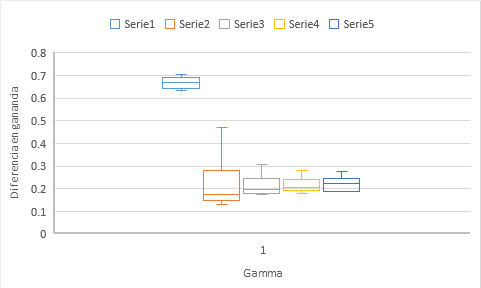
\includegraphics[scale=1]{Cajas1.png}
	\caption{Diagramas BoxPlot para la variable Gamma}
	\label{Cajas1}
\end{figure}

\begin{figure} [H]
	\centering
	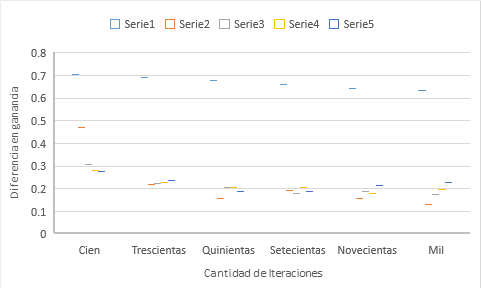
\includegraphics[scale=1]{Cajas1_1.png}
	\caption{Diagramas BoxPlot para la variable Iteraciones}
	\label{Cajas1_1}
\end{figure}

En estas figuras se ve la gran diferencia en los diagramas cuando se quiere observar media y varianza para cada valor, siendo razonable el resultado en los valores de gamma, donde lo que varía es el número de iteraciones, y tomadas como cinco valores aislados para cada valor en la cantidad de iteraciones, cuando la que variaba era gamma. Este comportamiento se debe a que al aumentar la cantidad de iteraciones en el experimento, se obtienen menores valores en la diferencia de las ganancias, mientras que al aumentar gamma, puede mejorar o empeorar el valor de la diferencia de las ganancias indistintamente.

Con los datos de la misma tabla \ref{experimento1}, se genera el análisis de varianza ANOVA, el cual se presta en la tabla \ref{tab:Anova1}. 

\begin{table}[H]
\centering\caption{ANOVA para Distancias en ganancias usando Gamma}
\small
\begin{tabular}{lrrrr}
\multicolumn{5}{c}{\textbf{ANÁLISIS DE VARIANZA}}             \\
\multicolumn{1}{c}{\textit{\textbf{\begin{tabular}[c]{@{}c@{}}Origen de las \\ \\ variaciones\end{tabular}}}} & \multicolumn{1}{c}{\textit{\textbf{\begin{tabular}[c]{@{}c@{}}Promedio de \\ \\ los cuadrados\end{tabular}}}} & \multicolumn{1}{c}{\textit{\textbf{F}}} & \multicolumn{1}{c}{\textit{\textbf{Probabilidad}}} & \multicolumn{1}{c}{\textit{\textbf{\begin{tabular}[c]{@{}c@{}}Valor crítico \\ \\ para F\end{tabular}}}} \\
                  & \multicolumn{1}{l}{}                                               & \multicolumn{1}{l}{}                    & \multicolumn{1}{l}{}                               & \multicolumn{1}{l}{}                                          \\
\textbf{Gamma}                                                                                                & 340127.902                                    & 16.7727717                              & 0.0000002762                                       & 2.602987403                                        \\
\textbf{Iteraciones}                                                                                             & 20273.7958                                       & 0.9997643429                            & 0.4382016733                                       & 2.602987403                                     
\end{tabular}
\label{tab:Anova1}
\end{table}

Para la primera variable, Gamma, se obtiene el valor de \textit{F} mayor al de \textit{F crítica} y una probabilidad muy baja $(P<0.05)$, lo que indica que existe una diferencia significativa en Gamma que afecta la variable dependiente.

Para la segunda variable, Iteraciones, se obtiene el valor de \textit{F} menor al de \textit{F crítica} y una probabilidad muy alta $(P>0.05)$, lo que indica que no existe una diferencia significativa en el número de iteraciones que afecta la variable dependiente.

